% LTeX: language=it

\section{Risoluzione del Problema}
Per la risoluzione del problema è possibile adottare due approcci che portano, sulla base della ipotesi fatte, a due diversi risultati.
Mentre una soluzione è solo una approssimazione ma di facile calcolo, l'altra è più precisa ma richiede l'uso di più formule e calcoli.

\subsection{Pallina da Ping Pong come Cubetto}
La prima soluzione è quella di considerare la pallina da ping pong come un cubetto di lato pari al diametro della pallina.
In questo modo, il volume della pallina è dato da:

\begin{equation}
    V_{pallinacubetto} = 0,04^3 = 64 cm^3
\end{equation}

Il numero di palline che possono starci nell'autobus è dato da:

\begin{equation}
    NP_{pallinacubetto} = \frac{V_{bus}}{VP_{pallinacubetto}} = \frac{60}{64*10^-6} = 937500
\end{equation}


\subsection{Pallina da Ping Pong come Sfera}
La seconda soluzione è quella di considerare la pallina da ping pong come una sfera.
In questo caso, si prende in considerazione anche l'impilabilità della singola pallina.
Per facilitare i conti e il processo logico, è comodo ora considerare la distribuzione nello spazio delle palline come all'interno di un solido cristallino CCC (Corpo Centrato Cubico).

\begin{figure}[H]
    \centering
    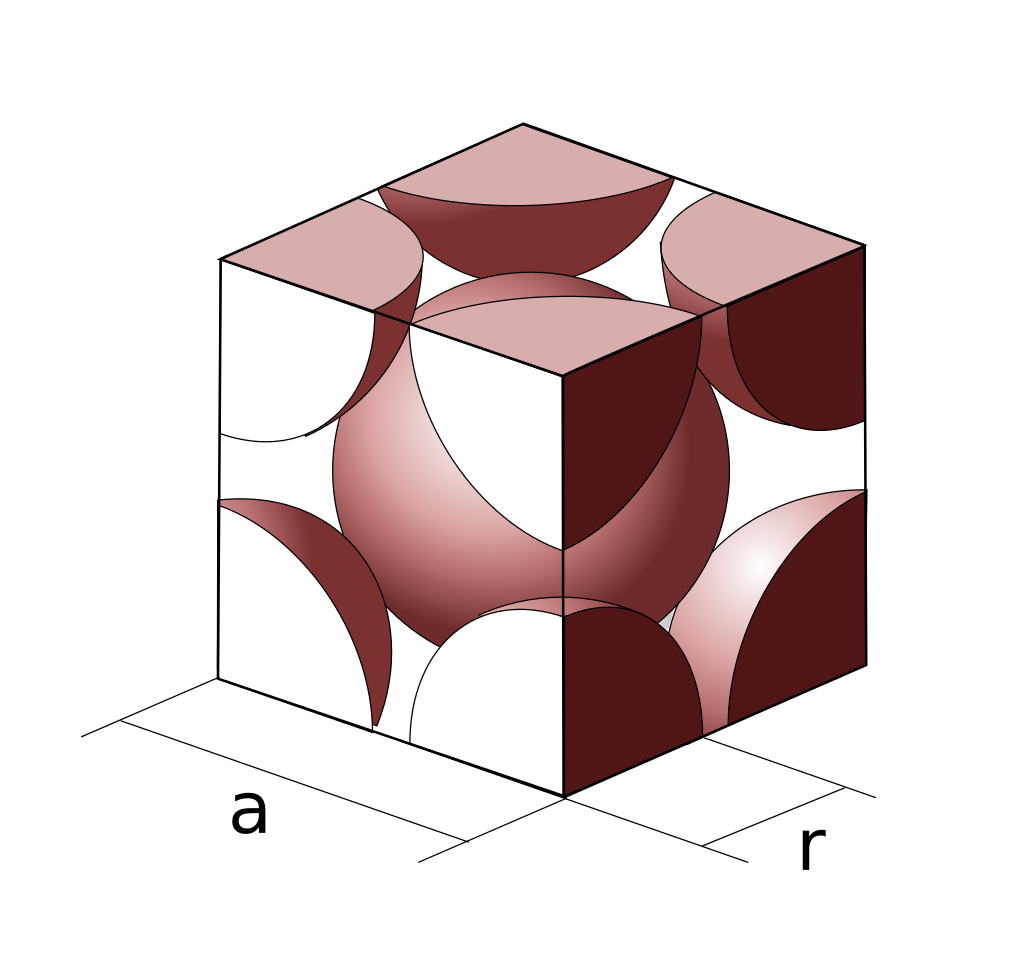
\includegraphics[width=.9\textwidth]{Modello_CCC}
    % \caption*{Fonte: https://it.wikipedia.org/wiki/Reticolo_cubico_a_corpo_centrato#/media/File:CCC_crystal_cell_(opaque).svg}
    \caption{Modello di distribuzione degli atomi in un solido cristallino CCC}
\end{figure}

Come si può vedere dalla figura, grazie a questo modello è possibile tenere conto dell'impilabilità delle palline.
In particolare, a livello di calcoli, si definisce il fattore di compattazione atomica (FCA) come:

\begin{equation}
    FCA = \frac{N_{atomi} * V_{atomo}}{V_{cella}}
\end{equation}

Dove:

\begin{itemize}
    \item $N_{atomi}$ è il numero di atomi presenti nella cella
    \item $V_{atomo}$ è il volume di un atomo
    \item $V_{cella}$ è il volume della cella che li contiene
\end{itemize}

Per semplici considerazioni goniometriche, si può dimostrare che il lato della cella è dato da:

\begin{equation}
    a = \frac{4 * R_{atomo}}{\sqrt{3}}
\end{equation}

Dove $R_{atomo}$ è il raggio dell'atomo (o della pallina di Ping Pong nel caso specifico).

Svolgendo i calcoli, si ottiene che $FCA = 0,68$.
Essendo poi il volume della cella dato da:

\begin{equation}
    V_{cella} = a^3 = \frac{64 * R_{atomo}^3}{3 * \sqrt{3}}
\end{equation}

Si ottiene che il numero di palline che possono starci nell'autobus è dato da:

\begin{equation}
    NP_{pallinasfera} = \frac{V_{bus}}{V_{pallina} * FCA} = \frac{60}{4 * 10^-6 * 0,68} = 1,102,941,176
\end{equation}